\documentclass{article}
\usepackage{amsmath}
\usepackage{bm}
\usepackage{graphicx}
\usepackage{appendix}

\title{Bayesian update rule leads to information theoretically optimal evolution\\ \begin{normalsize}Why to help those weaker than you\end{normalsize} }
\author{Tomas Ukkonen\\ \textrm{tomas.ukkonen@iki.fi} }
\date{\today}
\begin{document}
\maketitle

\section{Introduction} \label{introduction}

Evolution can be underatood as an optimization process that tries to collect information  \cite{infobook03} as well as possible from environment in order to increase fitness. One can think a current population as the distribution of genes $p(\mathbf{x})$ and then have a fitness function where outcomes are uncertain and defined as the probability of fitness $p(\mathbf{f}|\mathbf{x})$. It is then possible to use the bayes rule \cite{bdanalysis03} to calculate the posterior distribution of good genes $p(\mathbf{x}|\mathbf{f})$ given the fitness outcomes $\mathbf{f}$.

\begin{equation}
\label{bayesupdate}
p(\mathbf{x}|\mathbf{f}) \propto p(\mathbf{f}|\mathbf{x})p(\mathbf{x}) \end{equation}

\begin{equation}
\label{entropyupdate}
H(\mathbf{X}|\mathbf{F}) = H(\mathbf{X}) - I(\mathbf{X};\mathbf{F})
\end{equation}

The bayesian update rule is information theoretically optimal meaning information is gained as fast as possible from environment (Appendix \ref{information-theory}).

\section{Metropolis-Hastings and Evolution} \label{metropolis-hastings}

A paper published in 2003 \cite{strens03} describes methodology to combine genetic algorithms and Monte Carlo Markov Chain sampling. However, the author do not establish overall framework to combine bayesian inference, genetic algoritms and sampling discussed here.

Metropolis-Hastings method \cite{bdanalysis03} produces new samples $\{\mathbf{x}_{t+1}\}$ from a target distribution $P(\mathbf{x})$ by drawing samples $\{\mathbf{x}'\}$ from an auxiliary distribution $g(\mathbf{x}'|\mathbf{x}_t)$ and then accepting samples $\mathbf{x}'$ with probability $a$,

\begin{equation}
  \label{mcmcsampling1}
  a = min(1, \frac{P(\mathbf{x}')}{P(\mathbf{x}_t)} \frac{g(\mathbf{x}_t|\mathbf{x}')}{g(\mathbf{x}'|\mathbf{x}_t)})
\end{equation}.

To mimic the evolution, $\{\mathbf{x}'\}$s are drawn from a bayesian prior distribution $g(\mathbf{x}'|\mathbf{x}_t) = p(\mathbf{x}')$ and the target distribution is the posterior $P(\mathbf{x}) = p(\mathbf{x}|\mathbf{f})$. Straightforward calculation (also see Appendix \ref{detailed-balance}) then shows that the accepting probability $a$ becomes

\begin{equation}
  \label{mcmcsampling2}
  a = min(1, \frac{p(\mathbf{f}|\mathbf{x}')}{p(\mathbf{f}|\mathbf{x}_t)})
\end{equation}

So cases when a fitness likelihood ratio increases are always accepted and when it worsens, samples are still accepted with probability $a$. This mechanism, of 1) drawing samples from a prior $p(\mathbf{x})$, and then 2) accepting new samples according to the fitness likelihood ratio $a$, creates MCMC chain converging to the bayesian posterior assuming that significant convergence happens in a single iteration of Metropolis-Hastings rule and/or the limiting distribution is same for the each observation of $\mathbf{f}$. In practice, we have $M$ samples from $p(\mathbf{x})$ and we now need to generate more samples (``sex'') having the same distribution and then put them through fitness likelihood ratio (``soft competition'') so we get the proper posterior.
 
To further simplify generation of similarly distributed genomes through ``sex'', it is assumed that genes are independently distributed,

\begin{equation}
  p(x_1,x_2,...,x_n) = \prod_{i=1}^{N}p(x_i)
\end{equation}

This will then allow generating new similarly distributed genome from the two randomly chosen ``parent genomes'' $p(\mathbf{x}^k)$ and $p(\mathbf{x}^l)$ by choosing genes randomly from either one

\begin{equation}
  p(\mathbf{x}^{new}) = \prod_{i=1}^{N}p(x_i^{random(k,l)})
\end{equation}

A pool of $M$ individuals from the previous generation $\{\mathbf{x}_t\}$ is then generated and updated according to the modified Metropolis-Hastings sampling rule outlined above.


\section{Experiments} \label{experiments}

Three synthetic inference problems were used to test our theoretical framework.

\subsection{Experiment 1}

To investigate the implementation of the modified Metropolis-Hastings algorithm, $N=100$ bits long genome and a random initial population of size $M=100$ was genenerated where each bit in on position increases fitness score by one. The data likelihood probabilities for fitness was chosen to be binomial distribution 

\begin{equation}
  p(f|\mathbf{x}) = \binom{N}{f} p^{f}(1-p)^{N-f}, p = \frac{sum(\mathbf{x})}{N}
\end{equation}

and the observed fitness values $f$ were drawn from the same distribution as $p(f|\mathbf{x}')$. Computer simulations were run 30 times, each time simulating 1000 generations. In our experiments, the fitness failed to improve significantly at all (Figure \ref{fig:experiment1f3}) and a small alterations to the implementation didn't remedy the situation. After something like 500 iterations, inspection of binary genomes revealed that the whole population had become homogenous and each individual had the same genome.

\begin{figure}

\centering
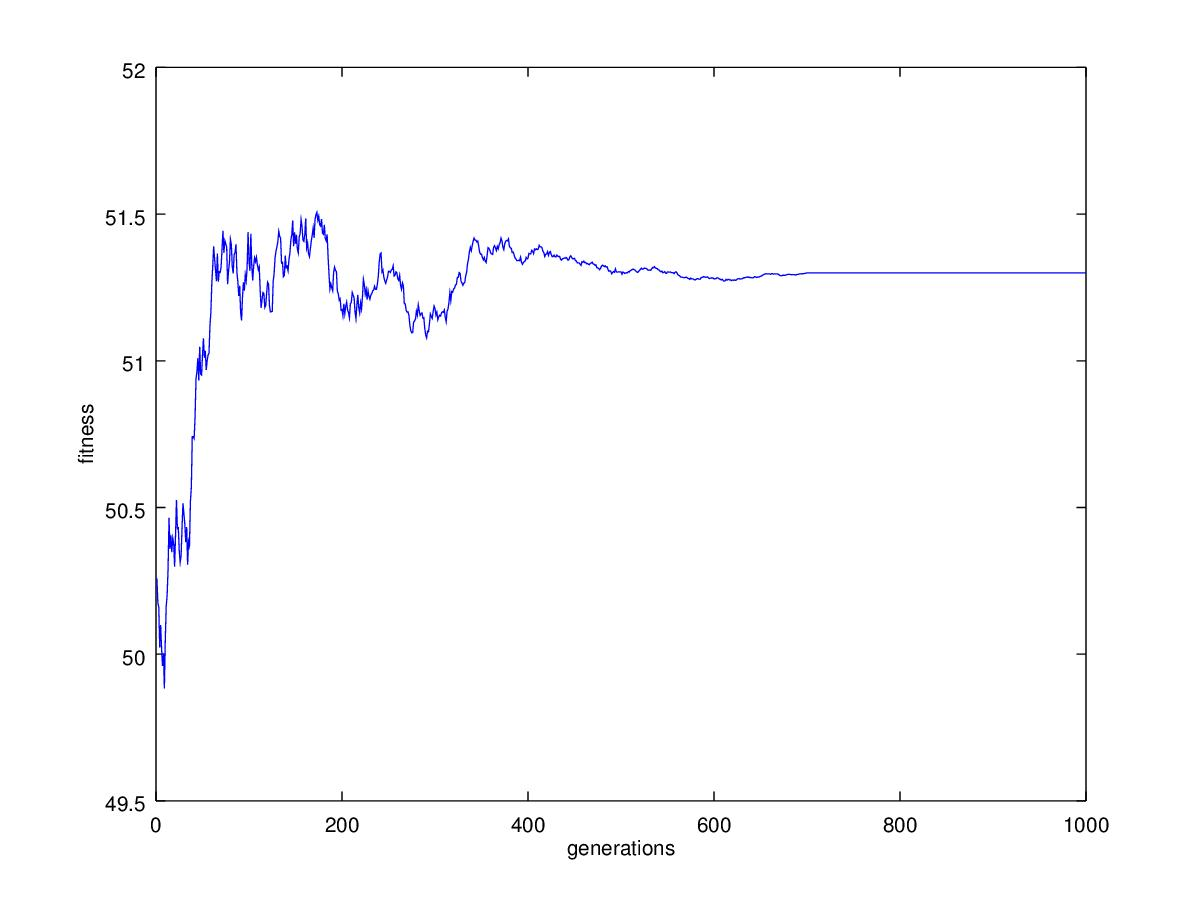
\includegraphics[keepaspectratio,width=0.9\textwidth]{experiment1figure3.jpg}

\caption{Average population fitness in Experiment 1}

\label{fig:experiment1f3}

\end{figure}


\subsection{Experiment 2}

Next, a much more direct fitness likelihood ratio function was tried. $N=20$ bits long genome and random initial population of size $M=100$ was generated. Fitness values $f$ were not directly used and instead a single probability value was used to calculate fitness likelihood ratio.


\begin{equation}
  \begin{aligned}
    \frac{p(f|\mathbf{x})}{p(f|\mathbf{x}_{t})} &= \frac{Bernoulli(f=1|p=\frac{sum(\mathbf{x})}{N})}{Bernoulli(f=1|p=\frac{sum(\mathbf{x}_{t})}{N})} \\
    \frac{p(f|\mathbf{x})}{p(f|\mathbf{x}_{t})} &= \frac{sum(\mathbf{x})/N}{sum(\mathbf{x}_{t})/N}
  \end{aligned}
\end{equation}

Computer simulations were run 30 times, each time simulating 100 generations which was enough for the convergence. To test speed of convergence, acceptance rate $a(k)$ was varied using different values of $k$ (Figures \ref{fig:experiment2_1}, \ref{fig:experiment2_10} and \ref{fig:experiment2_01}).

\begin{equation}
  \label{mcmcsampling3}
  a(k) = min(1, \frac{p(f|\mathbf{x}')}{p(f|\mathbf{x}_t)})^{k}
\end{equation}
r
The greater values of $k$ significantly reduced time to convergence as expected as more probability mass concentrates near peaks of distributions and there is less exploratory random walk behaviour (Figure \ref{fig:experiment2_10}).

\begin{figure}

\centering
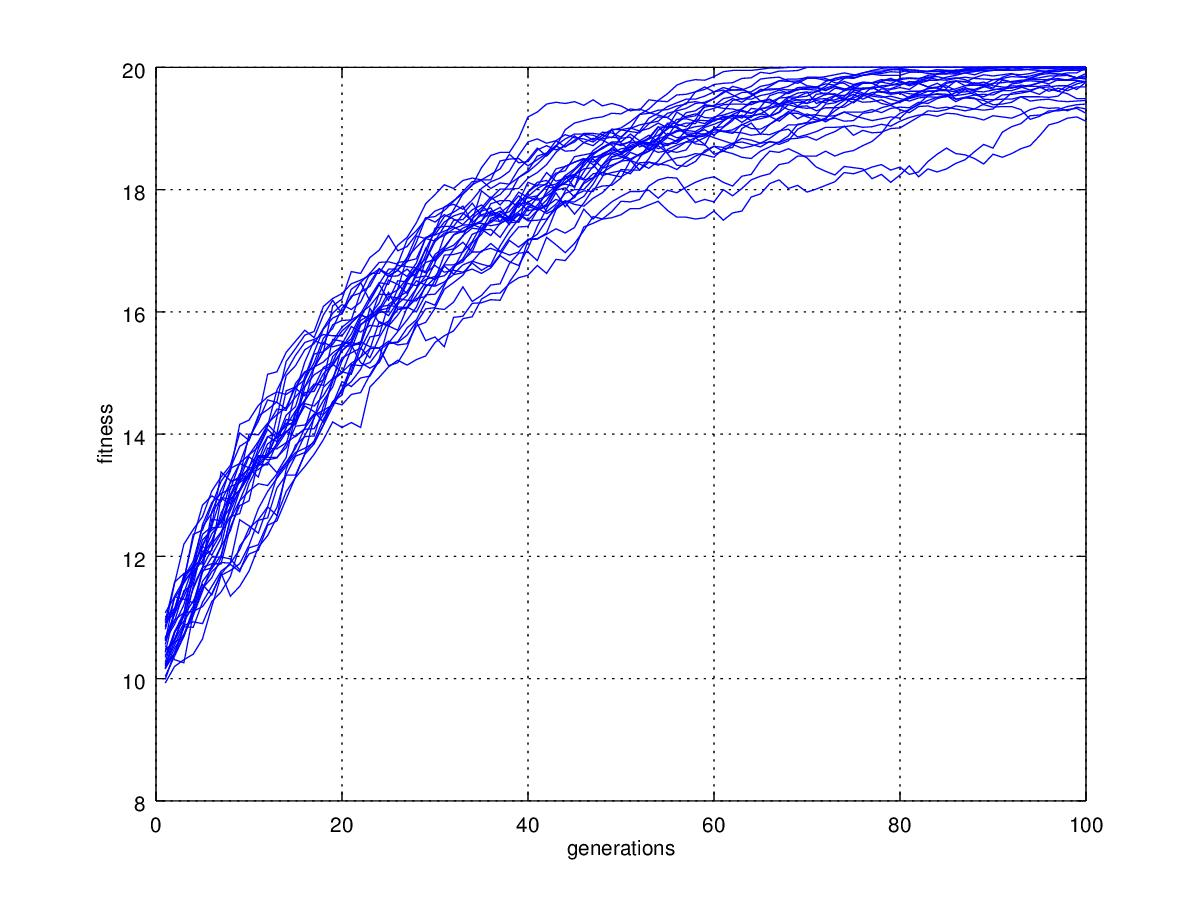
\includegraphics[keepaspectratio,width=0.9\textwidth]{experiment2figure2_1.jpg}

\caption{Average population fitness ($k = 1$) in Experiment 2}

\label{fig:experiment2_1}

\end{figure}

\begin{figure}

\centering
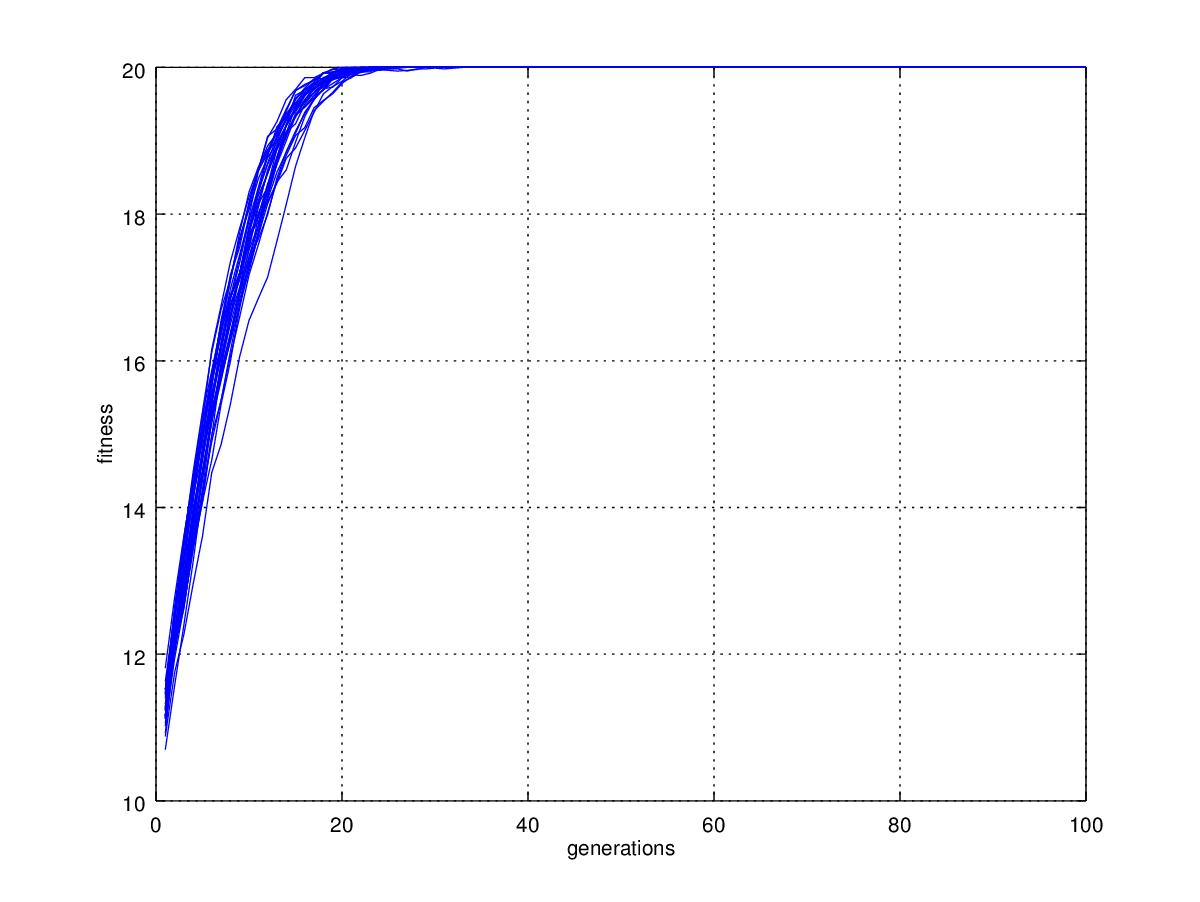
\includegraphics[keepaspectratio,width=0.9\textwidth]{experiment2figure2_10.jpg}

\caption{Average population fitness ($k = 10$) in Experiment 2}

\label{fig:experiment2_10}

\end{figure}

\begin{figure}

\centering
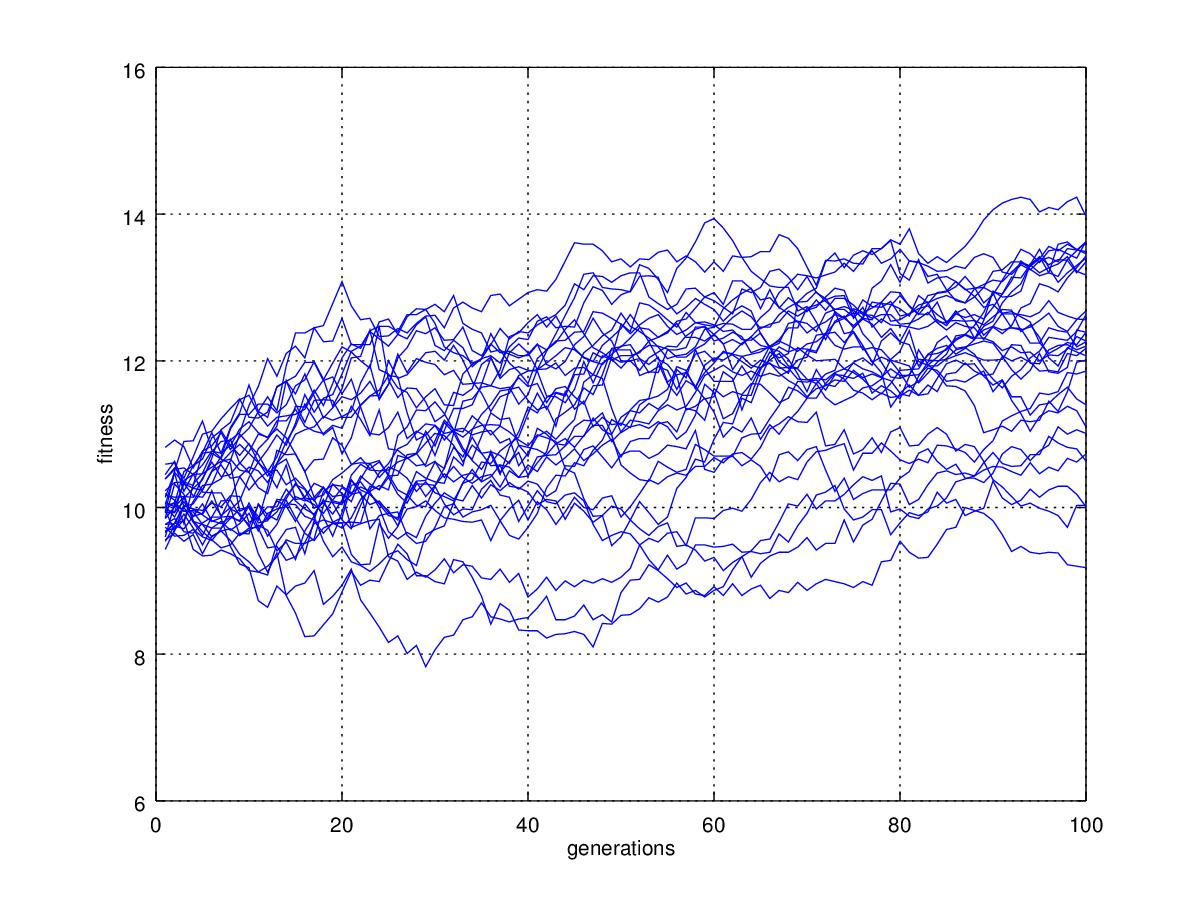
\includegraphics[keepaspectratio,width=0.9\textwidth]{experiment2figure2_01.jpg}

\caption{Average population fitness ($k = 1/10$) in Experiment 2}

\label{fig:experiment2_01}

\end{figure}


\subsection{Experiment 3}

While more aggressive competitional pressure (higher $k$ values) leads to significantly faster convergence in Experiment 2. It is likely that it will ``overfit'' solutions more easily by having unrealistical data likelihoods and fail to break free from local optimas. To investigate this, an alternative fitness likelihood distribution was chosen:

\begin{equation}
  p(f|\mathbf{x}) = 
  \begin{cases}  
    sum(\mathbf{x})/N & sum(\mathbf{x})/N \geq 0.5 \\
    1 - 0.95*sum(\mathbf{x})/N & sum(\mathbf{x})/N < 0.5 \\
  \end{cases}
  \label{alternative_fitness}
\end{equation}

It can be seen that Equation \ref{alternative_fitness} creates two different local optimums, one slightly more probable one, in which all bits are zero and, the second one, in which all bits are equal to one. Experiment is started from a position where 55\% the bits ($N=20$) are equal to one and closer to the slightly worse solution. Population size was again chosen to be $M=100$ and evolution was simulated for 500 generations.
By inspecting Figures \ref{fig:experiment3_1} and \ref{fig:experiment3_10} it is clear that larger choice of $k$ dampens tails of distributions causing optimization to converge faster. However, the larger $k$ also makes the process much more likely to get trapped into local maxima. A more lax choice of $k=1/10$ (Figure \ref{fig:experiment3_01}), on the other hand, allows sampling to find solutions close to the alternative (global) optimum ($f = 0$).

\begin{figure}

\centering
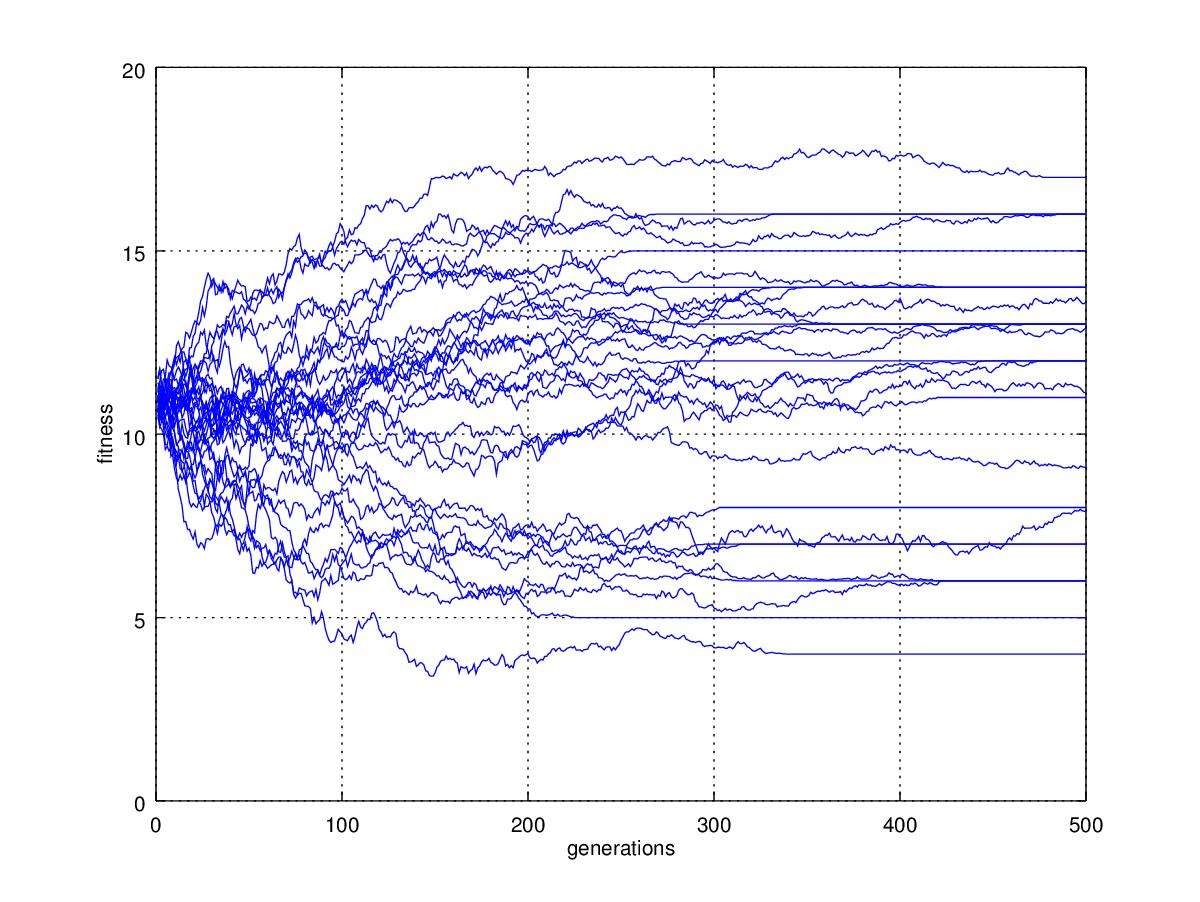
\includegraphics[keepaspectratio,width=0.9\textwidth]{experiment3figure2_01.jpg}

\caption{Average population fitness ($k = 1/10$) in Experiment 3}

\label{fig:experiment3_01}

\end{figure}

\begin{figure}
  
\centering
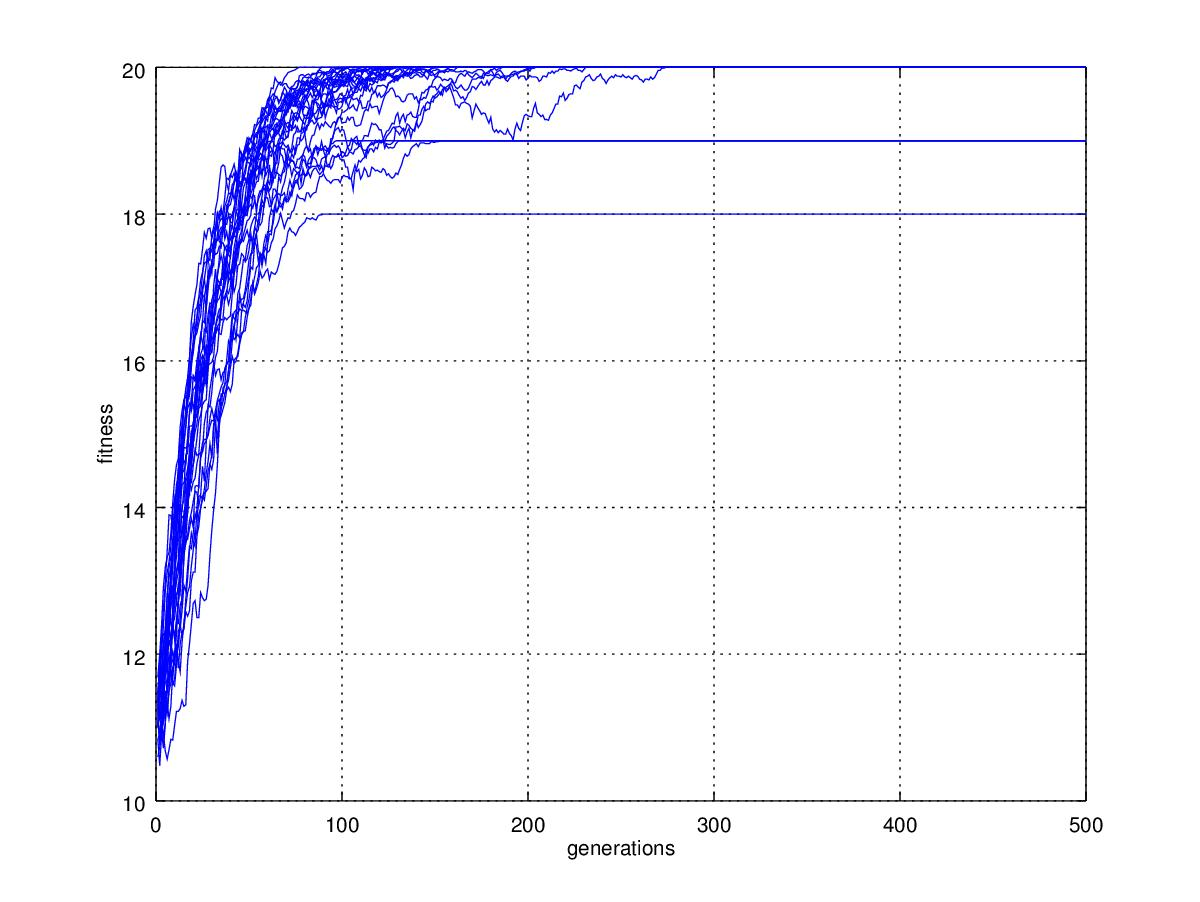
\includegraphics[keepaspectratio,width=0.9\textwidth]{experiment3figure2_1.jpg}

\caption{Average population fitness ($k = 1$) in Experiment 3}

\label{fig:experiment3_1}

\end{figure}


\begin{figure}

\centering
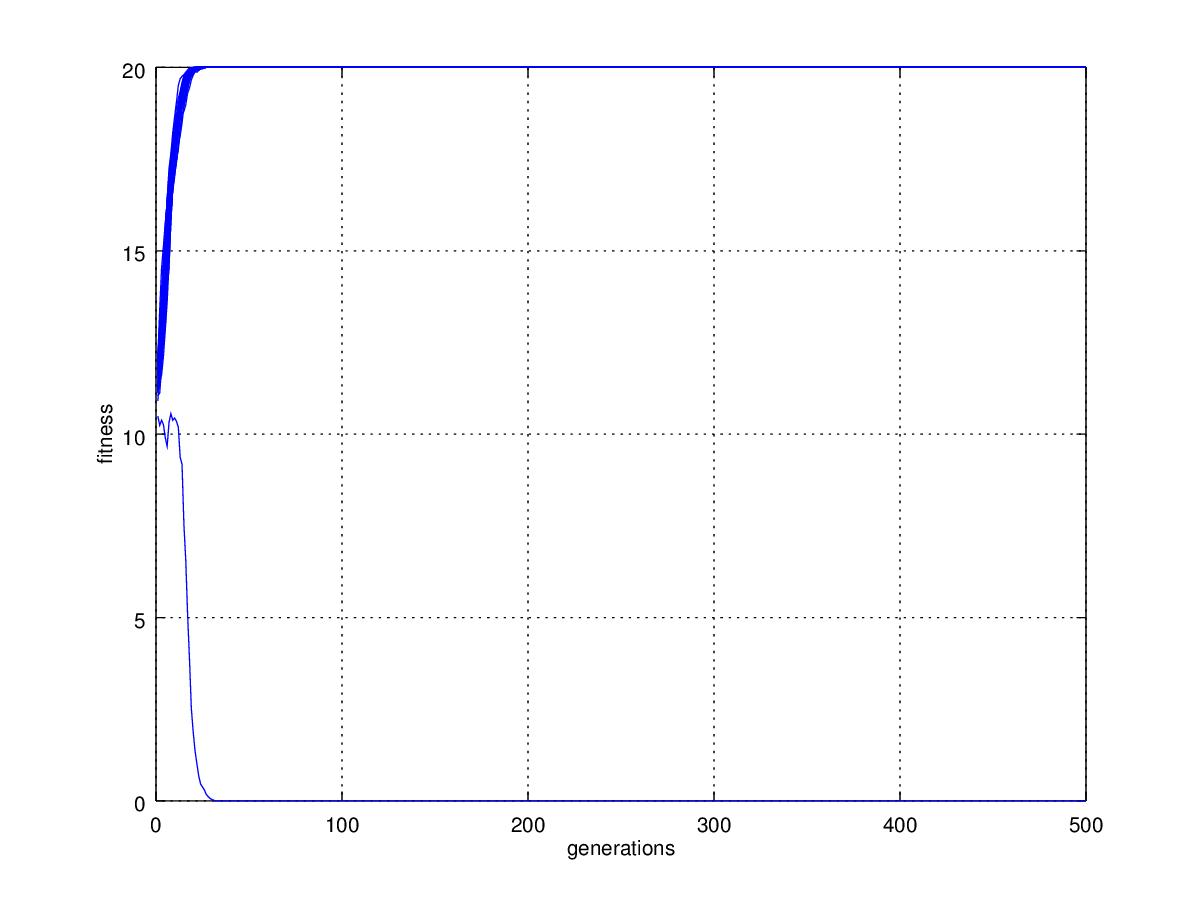
\includegraphics[keepaspectratio,width=0.9\textwidth]{experiment3figure2_10.jpg}

\caption{Average population fitness ($k = 10$) in Experiment 3}

\label{fig:experiment3_10}

\end{figure}


\section{Conclusions} \label{conclusions}

The keypoint is that in order to get good results and avoid getting stuck into local minimas, one needs to support individuals sampling low probability regions/tails of the distribution. If the individuals in low probability regions die, then the search and transfer of information doesn't happen as fast as possible and the group is likely to lose against other groups which are able to collect and process information faster. This means weaker individuals (risk takers) should be supported somehow in order to maintain the whole distribution and the inference/optimization rule. For example, stronger individuals (having enough intelligence) may gain information by observing and learning from mistakes of others. 

In this paper, evolutionary sampling framework is derived from Metropolis-Hastings MCMC sampling in Section \ref{metropolis-hastings} and it is shown to be information theoretically optimal. The resulting method for sampling bayesian posterior is similar to evolution and genetic algorithms. Further work could involve improved modelling, better computer simulations and finding proper balance between improved adaptation speed and resource use needed to support low fitness individuals.

\begin{thebibliography}{9}

\bibitem{infobook03}
  MacKay D.,
  \emph{Information Theory, Inference and Learning Algorithms},
  Cambridge University Press,
  2003.

\bibitem{bdanalysis03}
  Gelman A., Carlin J., Stern H. and Rubin D.,
  \emph{Bayesian Data Analysis. 2nd edition.},
  CRC Press, 
  2003.

\bibitem{strens03}
  Strens M.,
  \emph{Evolutionary MCMC Sampling and Optimization in Discrete Spaces},
  Proceedings of The Twentieth International Conference of Machine Learning,
  2003.

\bibitem{entropy01}
  Beirlant J., Dudewicz E., Györfi L., van der Meulen E.,
  \emph{Nonparametric entropy estimation: an overview},
  2001.

\end{thebibliography}


\appendix
\section{Information Theory} \label{information-theory}

It is easy to prove Equation \ref{entropyupdate} is correct from bayesian update Equation \ref{bayesupdate}.

\begin{equation*}
\begin{aligned}
  p(\bm{x}|\bm{f})p(\bm{f}) &= p(\bm{f}|\bm{x})p(\bm{x})\\
  log(p(\bm{x}|\bm{f})) + log(p(\bm{f})) &= log(p(\bm{f},\bm{x}))\\
  E_{\bm{x}\bm{f}}\{log(p(\bm{x}|\bm{f})) + log(p(\bm{f}))\} &= E_{\bm{x}\bm{f}}\{log(p(\bm{f},\bm{x}))\}\\  
  H(\bm{X}|\bm{F})+H(\bm{F}) &= H(\bm{X},\bm{F}) \\
  H(\bm{X}|\bm{F}) &= H(\bm{X},\bm{F}) - H(\bm{F}) \\
  H(\bm{X}|\bm{F}) &= H(\bm{X}) - I(\bm{X};\bm{F})
\end{aligned}
\end{equation*}

However, the reverse is not necessarily true.  There may be non-bayesian methods to process data that are information theoretically optimal as well.

\section{MCMC Sampling} \label{detailed-balance}

\subsection{Detailed Balance}

Necessarily condition for Monte Carlo Markov Chain to converge is detailed balance. The detailed balance means that transitions between states
$\mathbf{x}$ and $\mathbf{x}'$ must be reversible

\begin{equation}
  \pi(\mathbf{x})P(\mathbf{x}'|\mathbf{x}) = \pi(\mathbf{x}')P(\mathbf{x}|\mathbf{x}')
\end{equation}

where $\pi(\mathbf{x})$ is a limiting target distribution. This is achieved by assuming without loss of generality
$\frac{p(f|\mathbf{x}')}{p(f|\mathbf{x})} \leq 1$ and choosing a transfer probability to be 

\begin{equation} \label{transfer1}
  \begin{gathered}
    P(\mathbf{x}'|\mathbf{x}) = p(\mathbf{x}') a(\mathbf{x}'|\mathbf{x}) + \left(1 - \int p(\mathbf{x}') a(\mathbf{x}'|\mathbf{x}) \mathrm{d}\mathbf{x}'\right)\delta(\mathbf{x}' - \mathbf{x}) 
  \end{gathered}
\end{equation}

The latter term uses impulse function $\delta(\mathbf{x})$ to add rejection probability at $\mathbf{x}=\mathbf{x}'$. The reverse transfer probability ($\frac{p(f|\mathbf{x})}{p(f|\mathbf{x}')} \geq 1$) is 

\begin{equation} \label{transfer2}
  \begin{aligned}
    P(\mathbf{x}|\mathbf{x}') &= p(\mathbf{x}) \cdot a(\mathbf{x}|\mathbf{x}') \\
    P(\mathbf{x}|\mathbf{x}') &= p(\mathbf{x}) \cdot 1
  \end{aligned}
\end{equation}

The transfer probabilities are proper distributions and inserting Equations \ref{transfer1} and \ref{transfer2}
into the detailed balance equation ($\mathbf{x} \neq \mathbf{x}'$) gives 

\begin{equation} \label{detailed-balance-eq}
  \begin{aligned}
    \pi(\mathbf{x}) p(\mathbf{x}') \frac{p(f|\mathbf{x}')}{p(f|\mathbf{x})} &= \pi(\mathbf{x}')p(\mathbf{x}) \\
    \pi(\mathbf{x}) p(\mathbf{x}') p(f|\mathbf{x}') &= \pi(\mathbf{x}')p(\mathbf{x})p(f|\mathbf{x}) \\
    \pi(\mathbf{x}) p(\mathbf{x}') \frac{p(\mathbf{x}'|f)p(f)}{p(\mathbf{x}')} &= \pi(\mathbf{x}')p(\mathbf{x})\frac{p(\mathbf{x}|f)p(f)}{p(\mathbf{x})} \\
    \pi(\mathbf{x}) p(\mathbf{x}'|f) &= \pi(\mathbf{x}')p(\mathbf{x}|f)
  \end{aligned}
\end{equation}

The detailed balance is fulfilled in Equation \ref{detailed-balance-eq} by choosing $\pi(\mathbf{x}) = p(\mathbf{x}|f)$. It is then left to consider the case $\mathbf{x}' = \mathbf{x}$ where $a(\mathbf{x},\mathbf{x}) = 1$. The Equation \ref{transfer1} becomes 

\begin{equation} \label{transfer3}
  \begin{gathered}
    P(\mathbf{x}|\mathbf{x}) = p(\mathbf{x}) + \left(1 - \int p(\mathbf{x}') a(\mathbf{x}'|\mathbf{x}) \mathrm{d}\mathbf{x}'\right) 
  \end{gathered}
\end{equation}

This means the integral is one and $P(\mathbf{x}'|\mathbf{x}) = p(\mathbf{x}') a(\mathbf{x}'|\mathbf{x})$ is always a proper distribution. The limiting distribution $\pi(\mathbf{x})$, when $\mathbf{x}=\mathbf{x}'$, is then any proper distribution.


\end{document}

